\section{Lineare Zeitinvariante Systeme}
\begin{center}
  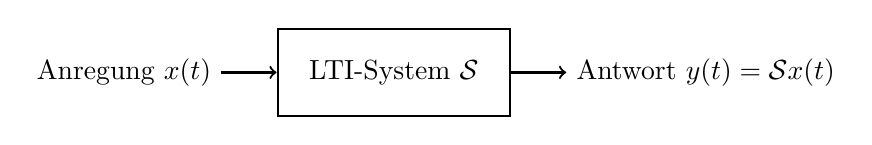
\begin{tikzpicture}[
      system/.style = {draw, thick, inner sep = .4cm}
    ]
    \node[system] (lti) {LTI-System \(\mathcal{S}\)};
    \draw[thick, ->] (lti.east) to ++(.7,0) node[right] {Antwort \(y(t) = \mathcal{S}x(t)\)};
    \draw[thick, ->] (lti.west) ++(-.7,0) node[left] {Anregung \(x(t)\)} to (lti.west);
  \end{tikzpicture}
\end{center}
Ein System mit der folgenden Eigenschaften ist als LTI bezeichnet.
\begin{center}
  \begin{tabularx}{\linewidth}{l >{\(\displaystyle }X<{\)}}
    Linear & \mathcal{S} (ax_1 + bx_2) = a\mathcal{S} x_1 + b\mathcal{S} x_2 = ay_1 + by_2 \\
    Zeitinvariant & \mathcal{S} x(t + t_0) = y(t + t_0) \\
  \end{tabularx}
\end{center}
LTI Systeme sind mit linearer DGL mit konstanten Koeffizienten mathematisch beschreibt.
\[
  x = \sum_{k=0}^n a_k y^{(k)} = a_n y^{(n)} + a_{n-1} y^{(n-1)}+ \cdots + a_0 y
\]
Der \(\mathcal{S}\) Operator entspricht mathematisch zu einer Faltung in
Zeitbereich mit der \emph{Gewichtsfunktion} \(g(t)\) oder einem Produkt im
Bildbereich mit der \emph{\"Ubertragungsfunktion} \(G(s) = \mathcal{F} g(t)\)
(Faltungssatz).
\[
  \mathcal{S}x(t) \equiv g(t) * x(s) \qquad \mathcal{S}X(s) \equiv G(s) \cdot X(s)
\]

\subsection{Impulsantwort}
\subsection{Frequenzgang}
\subsection{Eigenschwingungen}
\subsection{Station\"are L\"osung}
